\documentclass{beamer}
\usepackage[magyar]{babel}
\usepackage[utf8]{inputenc}
\usepackage[T1]{fontenc}
\usepackage{graphicx, tikz}
\usepackage[framemethod=TikZ]{mdframed}
\usepackage[version=4]{mhchem}

\bibliographystyle{apalike}


\mode<presentation>
{
    \usetheme{Boadilla}
    \usecolortheme{default}
    \usefonttheme{default}
    \setbeamertemplate{navigation symbols}{}
    \setbeamertemplate{caption}[numbered]
} 


\def\rar{\rightarrow}
\def\lar{\leftarrow}

\newcommand\quo[1]{``#1''}
\newcommand\subt[2]{#1_{\text{#2}}}
\newcommand\pard[2]{\frac{\partial #1}{\partial #2}}
\newcommand\abs[1]{\left|#1\right|}


\newcommand\inc[1] {
    \includegraphics[width=\textwidth]{#1}
}

\newcommand\img[2] {
    \includegraphics[width=#2\textwidth]{#1}
}

\newenvironment{ffig}[1]
{
    \begin{mdframed}[linecolor=#1, linewidth=5.0pt, roundcorner=5pt,
                     innerrightmargin=10pt, innerleftmargin=10pt,
                     innertopmargin=0pt, innerbottommargin=5pt,
                     skipabove=0pt, skipbelow=0pt,
                     backgroundcolor=white, frametitle={}, align=center]
    \begin{center}
}
{
    \end{center}
    \end{mdframed}
}

\newenvironment{fig}[1]
{
    \begin{minipage}{#1\textwidth}
    \begin{center}
}
{
    \end{center}
    \end{minipage}
}


\newcommand{\fcap}[1] {
    \captionof{figure}{#1}
}

\newcommand{\genenv}[1] {
    \def\b#1 { \begin{#1} }
    \def\e#1 { \end{#1} }
}


\def\bffig { \begin{ffig} }
\def\effig {   \end{ffig} }

\def\bfig { \begin{fig} }
\def\efig {   \end{fig} }

\def\bitz { \begin{itemize} }
\def\eitz {   \end{itemize} }

\def\bmini { \begin{minipage} }
\def\emini {   \end{minipage} }

\def\bcent { \begin{center} }
\def\ecent {   \end{center} }

\newcommand\annotatedFigureBoxCustom[8]{
    \draw[#5,ultra thick,rounded corners] (#1) rectangle (#2);
    \node at (#4) [fill=#6,thick,shape=circle,draw=#7,
                   inner sep=2pt,font=\sffamily,text=#8]
                   {\textbf{#3}};
}


% {from}{to}{text}{color}
\newcommand\anbox[4]{\annotatedFigureBoxCustom{#1}{#2}{#3}{#1}{#4}{white}{black}{black}}


\newcommand\antext[5]{
    \draw[#4, fill=#5, ultra thick, rounded corners] (#1) rectangle (#2)
    node[pos=0.5, font=\sffamily, text=black] {\textbf{#3}};
}


\newenvironment{anfig}[1]
{
    \begin{mdframed}[linecolor=blue!65!white, linewidth=2pt, roundcorner=0.75pt,
                     innerrightmargin=0.05pt, innerleftmargin=0.05pt,
                     innertopmargin=0.05pt, innerbottommargin=0.05pt, frametitle={}]
    \begin{tikzpicture}
    \node[anchor=south west,inner sep=0] (image) at (0,0)
    {\includegraphics[width=\textwidth]{#1}};
    \begin{scope}[x={(image.south east)},y={(image.north west)}]
}
{
    \end{scope}
    \end{tikzpicture}
    \end{mdframed}
}

\def\fcol{\color{blue!55!black}}

\newcommand{\fig}[1]{
    \begin{mdframed}[linecolor=blue!65!white, linewidth=1.75pt, roundcorner=0.75pt,
                     innerrightmargin=0pt, innerleftmargin=0pt,
                     innertopmargin=0pt, innerbottommargin=0pt,
                     backgroundcolor=white, frametitle={}, align=center]
        \includegraphics[width=1.0\textwidth]{#1}
    \end{mdframed}
}

\newcommand{\figm}[2]{
    \begin{center}
    \begin{minipage}[c]{#2\textwidth}
    \begin{mdframed}[linecolor=blue!65!white, linewidth=1.75pt, roundcorner=0.75pt,
                     innerrightmargin=0pt, innerleftmargin=0pt,
                     innertopmargin=0pt, innerbottommargin=0pt,
                     backgroundcolor=white, frametitle={}, align=center]
        \includegraphics[width=1.0\textwidth]{#1}
    \end{mdframed}
    \end{minipage}
    \end{center}
}

\newenvironment{minic}[1]
{
    \begin{center}
    \begin{minipage}[c]{#1\textwidth}
}
{
    \end{minipage}
    \end{center}
}


\newenvironment{figp}[4]
{
    \begin{minipage}[c]{#3\textwidth}
    \centering
    #1
    
    #2
    \end{minipage}
    \begin{minipage}[c]{#4\textwidth}
}
{
    \end{minipage}
}


\newcommand{\figc}[2]
{
    \begin{center}
    \begin{mdframed}[linecolor=blue!65!white, linewidth=1.75pt, roundcorner=0.75pt,
                     innerrightmargin=0pt, innerleftmargin=0pt,
                     innertopmargin=0pt, innerbottommargin=0pt,
                     backgroundcolor=white, frametitle={}, align=center]
    
    \includegraphics[width=1.0\textwidth]{#1}
    \end{mdframed}
    #2
    \end{center}
}

\newcommand\sepframe[1] {
    \begin{frame}
        \begin{center}
            \Huge \fcol
            #1
        \end{center}
    \end{frame}
}

\def\SubdLithoVelo{Subducted Lithospheric Slab Velocity Structure - George Helffrich}

\newcommand\sepcite[2] {
    \begin{frame}
        \begin{center}
            \Huge \color{blue!55!black}
            #1
            
            \cite{#2}
        \end{center}
    \end{frame}    
}

\newcommand\paper[2]{
    Title: #1 \\
    Author: #2
}



\graphicspath{{../images/}}

\title[Szubdukált lemez geofizikája]{Szubdukált lemez és köpenyék geofizikája}
\author{Bozsó István}
\institute[MTA CSFK GGI]{MTA CSFK Geodéziai és Geofzikai Intézet}
\date{2018.11.19.}

\begin{document}

\begin{frame}
    \titlepage
\end{frame}


\begin{frame}{A lemezvándorlás és szubdukció felfedezése elmélete}
    Horváth Ferenc: Wegener-centeráium: Megszületett-e a kontinensvándorlás Newtonja? \cite{horvath}
    \vspace{10pt}
    
    \pause
    
    \begin{center}
    \begin{minipage}[c]{0.625\textwidth}
        \centering
        \fig{horvath_ferenc.png}
        
        Horváth Ferenc (1944.03.24.-2018.11.17.)
    \end{minipage}
    \end{center}
\end{frame}


\begin{frame}{Wegener elmélet}
    \begin{itemize}
        \item \textbf{Alfred Wegener} (1880-1930)
        \begin{itemize}
            \item 1912 január 6. német Földtani Társulat ülése, Farnkfurt: ``A földkéreg nagyformáinak (a kontinensek és az óceánok) alakulásageofizkai adatok alapján''
            \item 1912 január 10. Marburg: ``A kontinensek horizontális elmozdulása''
            \item 1912-ben két publikáció
            \item ``...a kontinesvándorlás Newtonja még nem született meg'' 1929
        \end{itemize}
    \end{itemize}
\end{frame}


\begin{frame}{Wegener modellje}
    \begin{center}
        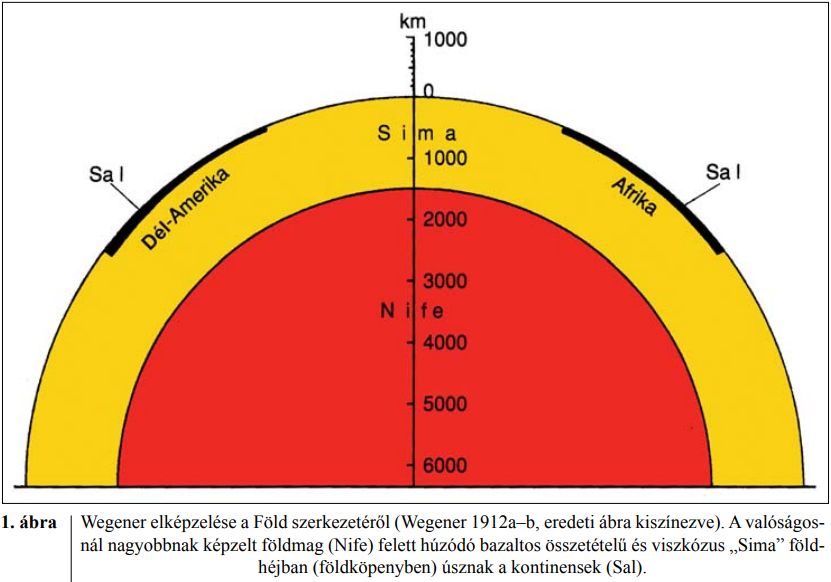
\includegraphics[width=0.525\textwidth]{wg_theory.png}
    \end{center}

    \begin{minipage}[c]{0.45\textwidth}
        \begin{itemize}
            \item kontinensek (Sal) belemerülnek és úsznak a földköpenyben (``Sima'')
            \item Sima vagy magma: bazaltos összetételű, viszkózus
            \item Nife: földmag
        \end{itemize}
    \end{minipage}
    \begin{minipage}[c]{0.45\textwidth}
    \begin{itemize}
        \item lehetséges hajtóerők
        \begin{itemize}
            \item Eötvös-erő (``Polflucht'')
            \item árapálysúrlódás
            \item köpenyáramlás
        \end{itemize}
    \end{itemize}
    \end{minipage}
\end{frame}


\begin{frame}{Lehetséges hajtóerők}
    \begin{figp}{\inc{wg_eotvos.png}}{}{0.47}{0.4}
        \begin{itemize}
            \item Eötvös Loránd fedezte fel (1905), $\ne$ Eötvös-effektus
            \item Föld- és potenciálfelületek alakja ellipszoid
            \item súlyerő vagy nehézségi erő (C) + ellenerő (T) $\rar$ egyenlítő felé mutató erő
        \end{itemize}
    \end{figp}
\end{frame}


\begin{frame}{Lehetséges hajtóerők}
    \begin{minipage}[c]{0.575\textwidth}
        \centering
        \inc{wg_tide.png}
    \end{minipage}
    \begin{minipage}[c]{0.35\textwidth}
        \begin{itemize}
            \item árapálymaximum $\ne$ Föld-Hold tömegközéppont egyenes
            \item Föld forgásának folyamatos lassítása, nyugati drift
            \item szilárd Föld, hidroszféra, atmoszféra nem tökéletesen rugalmas (viszkoelasztikus) $\rar$ 2-3$^\circ$ eltérés keletebbre
        \end{itemize}
    \end{minipage}
\end{frame}


\begin{frame}{Lehetséges hajtóerők}
    \begin{figp}{\inc{wg_cont_drift.png}}{Wegener elmélete a kontinensek vándorlásáról.}{0.45}{0.4}
        \begin{itemize}
            \item köpenyben radioaktív hőtermelés $\rar$ konvektív áramlás
            \item felfelé áramlás $\rar$ óceánközepi-hátság
            \item ütköző kontinensek $\rar$ lánchegységek
            \item lehetséges erőhatások nagyon kicsik $\rar$ ``sima'' teljesen viszkózus (folyadékszerű) viselkedés
            \item kis erők $\rar$ kis elmozdulások $\rar$ geológiai időskálákon, nagy elmozdulás
        \end{itemize}
    \end{figp}
\end{frame}


\begin{frame}{A kontinensvándorlás elmélet kritikusa}
    \begin{itemize}
        \item \textbf{Harold Jeffreys} (1891-1989); matematikus, csillagász, geofizikus; Naprendszer kialakulás, Föld belső szerkezet
        \item mag külső héja folyadékszerű (nincs nyíróhullám)
        \item Föld többi része szilárd, nyíróhullámok jelenléte $\rar$ minden erőhatás deformációval kompenzálódik
        \item Wegener féle erőhatások $\ll$ köpeny szakítási szilárdsága
        \item Jeffreys: A Földön minden hőmérséklet- és nyomáskülönbség már régen kiegyenlítődött
    \end{itemize}
\end{frame}


\begin{frame}{A Wegener elmélet támogatói - geológusok, fizikusok}
    \begin{itemize}
        \item \textbf{John Joly} (1857-1933); fizikus, természetes radioaktivitás;
        \item Kelvin földmodell (térben homogén paraméterek, konduktív hőterjedéssel hülő Föld), 96 (30) Ma $\leftrightarrow$ geológiai ismeretek
        \item együttműködés Rutherforddal, devon korú kőzetek korolása; 400 Ma (1913)
        \item nagytektonikai folyamatok energiája radioaktív hőtermelésből
        \item radioaktív elemek hőtermelése $\rar$ fokozatosan felhalmozódó hő $\rar$ ciklikus (100-200 Ma) bazaltömlés (ma ``forró folt'' vulkanizmus)
        \item bazaltos köpenyanyag áramlása a felszínre $\rar$ kontinesek vándorlása
    \end{itemize}
\end{frame}


\begin{frame}{A Wegener elmélet támogatói - geológusok, fizikusok}
    \begin{itemize}
        \item \textbf{Arthur Holmes} (1890-1965); geológus;
        \item radioaktív- és egyéb kormeghatározások $\rar$ Föld kora: 1600 Ma
        \item egyetértett Joly érvelésével
        \item ``...meggyőző bizonyítékaink vannak, amelyek a kontinesek egykori vándorlására mutatnak, mégpedig úgy, ahogy azt Wegener javasolta''
        \item Emile Argand (1879-1940): ``Mi nem szándékozunk a tektonikát visszavezetni a fizikára, ez a jövő feladata.''
    \end{itemize}
\end{frame}


\begin{frame}{A Wegener elmélet támogatói - geológusok, fizikusok}
    \begin{itemize}
        \item \textbf{Frank B. Taylor} (1860-1938); Harvard Egyetem tanulmányok: geológia, asztronómia; Amerikai Földtani Szolgálat (USGS) glaciológiai osztálya;
        \item kontinesek egyenlítő felé mozgása $\rar$ alpi-himalája-melanéziai és cirkum-pacifikus hegységrendszer kialakulására (1910)
        \item Eötvös-erő hatása? megfelelően nagy?
    \end{itemize}
    
    \begin{itemize}
        \item \textbf{W. Lambert} (1879-1968); USGS, geodéta;
        \item Eötvös-erő nagyságának kiszámítása: 30$^\circ$ északi szélességen 1 km átmérőjű kéregsűrűségű gömb
        \item súrlódásmentes gördülés 4-5 m/s átlagsebesség
        \item ha köpeny anyag folyadékszerű $\rar$ geológiai időskálán ezer km-es mozgások
    \end{itemize}
\end{frame}


\begin{frame}{A Wegener elmélet támogatói}
    \begin{minic}{0.95}
        \centering
        \inc{wg_taylor_theory.png}
    \end{minic}
\end{frame}


\begin{frame}{A Wegener elmélet támogatói - geológusok, fizikusok}
    \begin{itemize}
        \item \textbf{Reginald A. Daly} (1871-1957); tanulmányok: Torontói Egyetem, Harvard, Heidelberg, Párizs; MIT fizikai geológia; Harvard Egyetem: a geológia professzora;
        \item Lambert legfőbb támogatója; kontinesvándorlást hajtó mechanizmus keresése
        \item négy lehetséges hajtóerő
        \begin{itemize}
            \item árapálysúrlódás $\rar$ nyugati drift
            \item geoszinklinális mélyáramlások
            \item Eötvös-erő
            \item orogenezis során kialakuló feszültség
        \end{itemize}
        \item szerinte: egyik erő sem elegendő; többet kell tudni a földi anyagok reológiájáról
    \end{itemize}
\end{frame}

\begin{frame}{A Wegener elmélet támogatói - geológusok, fizikusok}
    \begin{itemize}
        \item \textit{Dél-Afrikai expedíció} Carnegie Intézet támogatásával Bushweld magmás komplexum (1922)
        \item Reginald A. Daly, F. Wright (1877-1953) petrológus, G. Molengraaf (1860-1942) delfti professzor, Alexander du Toit (1878-1948) geológus;
        \item Daly és Wright meggyőzése a kontinensvándorlás elmélet helyességéről; ``lobbizás'' $\rar$ Carnegie Intézet anyagi támogatása du Toit Dél-Amerika, Karoo Formáció feltárása
        \item adatok feldolgozása $\rar$ Dél-Afrika és Dél-Amerika karbon-jura képződményei, rétegtani, őslénytani, kőzettani hasonlóságok $\rar$ két kontinens karbontól összetartozott, középső jura szétszakadás
        \item bizonyíték a kontinesvándorlásra
    \end{itemize}
\end{frame}


\begin{frame}{A Wegener elmélet bizonyítékai}
    \begin{minipage}[c]{0.525\textwidth}
        \inc{wg_daly_theory.png}
    \end{minipage}
    \begin{minipage}[c]{0.45\textwidth}
        \begin{itemize}
            \item geoszinklinálisokban folyamatosan felhalmozódó üledék $\rar$ kéreg betüremkedik a folyadékszerű bazaltba (``glassy basalt'')
            
        \end{itemize}
    \end{minipage}
    \begin{itemize}
        \item bazalt peremek felé mozog $\rar$ peremek emelkednek $\rar$ üledék behordása
        \item mélyebbre süllyedő kéreg felmelegedik $\rar$ gyökér destabilizálódik, kiszakad, lesüllyed
        \item szabad térbe benyomul az emelt kéregrész $\rar$ üledéket felgyűri $\rar$ hegységképződés
    \end{itemize}
\end{frame}


\begin{frame}{A Wegener elmélet bizonyítékai}
    \begin{itemize}
        \item \textbf{William Bowie} (1872-1940), USGS geodéziai osztály vezetője;
        \item ``... a világ csillagászai és geodétái elhatározták, hogy pontos tesztmérésekkel ellenőrzik Wegener hipotézisét'' (New York Times, 1925)
        \item világméretű háromszögelés hálózat, rádiohullámok futási ideje $\rar$ kontinensek elmozdulása
        \item hibaszámítások: pontosság néhány m/év sebesség kimutatására nem elegendő (Oroskes 1999)
    \end{itemize}
\end{frame}


\begin{frame}{A Wegener elmélet bizonyítékai}
    \begin{itemize}
        \item \textbf{Felix Vening Meinesz} (1887-1966); holland mérnök, nemzeti geodéziai szolgálat; tengeri gravitációs mérések
        \item speciális kettős inga kifejlesztése, enyhén ingatag talapzaton is működőképes
        \item holland haditengerészet tengeralattjárója (1923-1927); több száz tenger alatti mérés
        \item mélytengeri Jáva-árok: -120, -140 mgal anomális (kontinentális terület, izosztatikus kompenzáció miatt $\pm$ 10-30 mgal)
        \item mélytengeri árok mentén kompressziós kéregbetüremkedés
        \item Carnegie Intézet, tengeralattjáró: Karib-árok mentén méresek (1932-1937); hasonló negatív gravitációs anomália
        \item mérésekben részt vettek: \textbf{Harry Hess} (1906-1969), \textbf{Maurice Ewing} (1906-1974) II.vh alatt mérések, 60-as években lemeztektonika megszületésénél fontos szerep
    \end{itemize}
\end{frame}


\begin{frame}{A lemeztektonikától napjainkig}
    \begin{itemize}
        \item Harry Hess gravitációs mérések $\rar$ árkoknál betüremkedő réteg modellje $\rar$ óceáni kéreg és a köpeny is mozog, ütközik és gyűrődik
        \item Harry Hess: ócáni aljzat szétterülésének elmélete (ocean-floor spreading) (1962)
        \item kontinensek litoszférán utazó, óceáni területekhez kapcsolódó lemezek részei, amelyek a részlegesen olvadt aztenoszférán mozognak
        \item megszületett a lemeztektonika elmélete
    \end{itemize}
\end{frame}


\begin{frame}{A lemezmozgás dinamikája}
    \begin{minic}{0.68}
        \centering
        \inc{wg_slab_mechanics.png}
    \end{minic}
    $F_{\text{SU}}$, $F_{\text{SP}}$: ``árokszívás'', indukált köpenyáramlás húzó hatása; $R_{\text{R}}$: lemez és asztenoszféra - súrlódás; $R_{\text{B}}$ alátolódó lemez hajlításához szükséges feszültség; $R_{\text{S}}$ felső köpenyben, mélységgel növekvő viszkozitás, sűrlódási ellenállás; $R_{\text{O}}$ kontinentális- és alátolódó lemez - súrlódás; $R_{\text{DO}}$, $R_{\text{DC}}$: óceáni- és kontinetális lemez, asztenoszféra köpenyáramlás súrlódás
\end{frame}


\begin{frame}{A lemezmozgás dinamikája}
    \begin{center}
        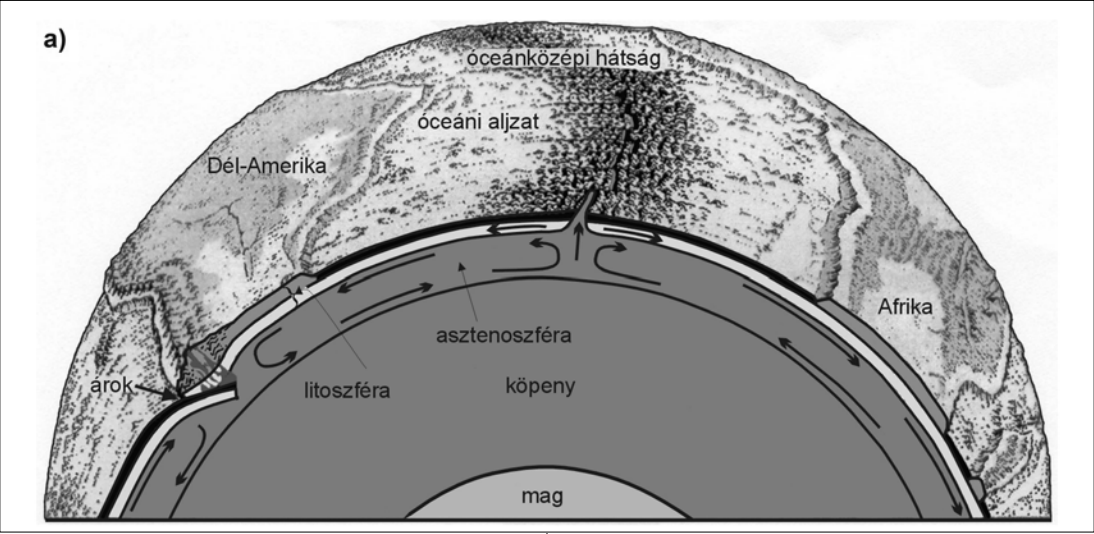
\includegraphics[width=0.85\textwidth]{wg_cell_flow.png}
    \end{center}
    \begin{itemize}
        \item lemeztektonika kezdeti időszakáig a köpenyáramlást tekintették a legfőbb mozgatóerőnek
        \item cellaszerű áramlás
        \item feláramlás: hátságoknál lemezek távolítása; leáramlás: lemezeket lefelé húzza
    \end{itemize}
\end{frame}


\begin{frame}{A lemezmozgás dinamikája}
    \begin{center}
        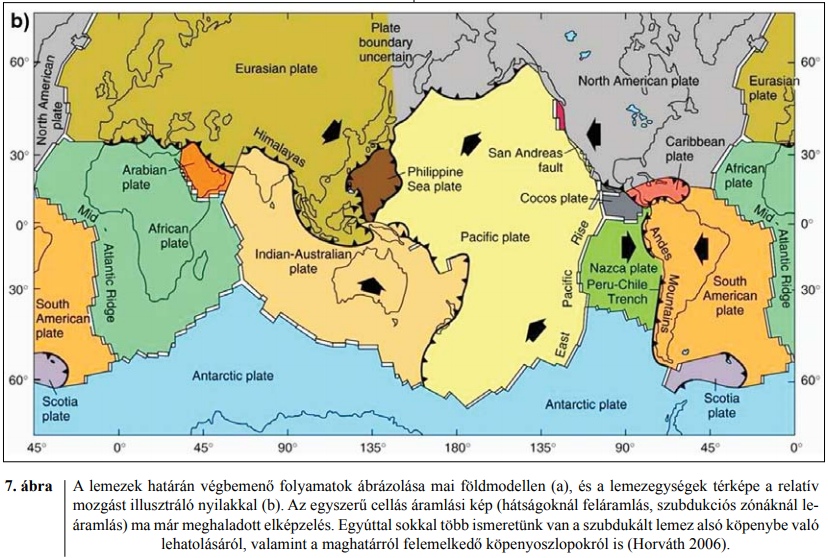
\includegraphics[width=0.95\textwidth]{wg_global_plate_movement.png}
    \end{center}
\end{frame}


\begin{frame}{A lemezmozgás dinamikája}
    \begin{itemize}
        \item hátságok mélytengeri árkok bonyolult geometria $\rar$ szabálytalan áramlási cella geometria
        \item hátságok helyzete nem fix, mélytengeri árkokhoz képest változó
        \item Antarktiszi-lemez növekedik, hátságok magukat tólják el az Antarktisztól?
        \item Kelet-Pacifikus-hátság Kalifornia déli részénél eltűnik; 30 Ma ezelőtt 1000 km-el nyugatabbra helyezkedett el
        \item hátságok központi hasadékvölgye = szakadási vonal a litoszférában, lemezekkel együtt mozog; asztenoszféra anyagának felszínre törése
    \end{itemize}
\end{frame}


\begin{frame}{A lemezek mozgásának abszolút sebessége}
    Forsyth és Uyeda (1975); köpeny hőoszlopok (mantle plumes) és forró folt (hot spot) mint abszolút koordinátarendszer fix pontjai
    
    \begin{center}
        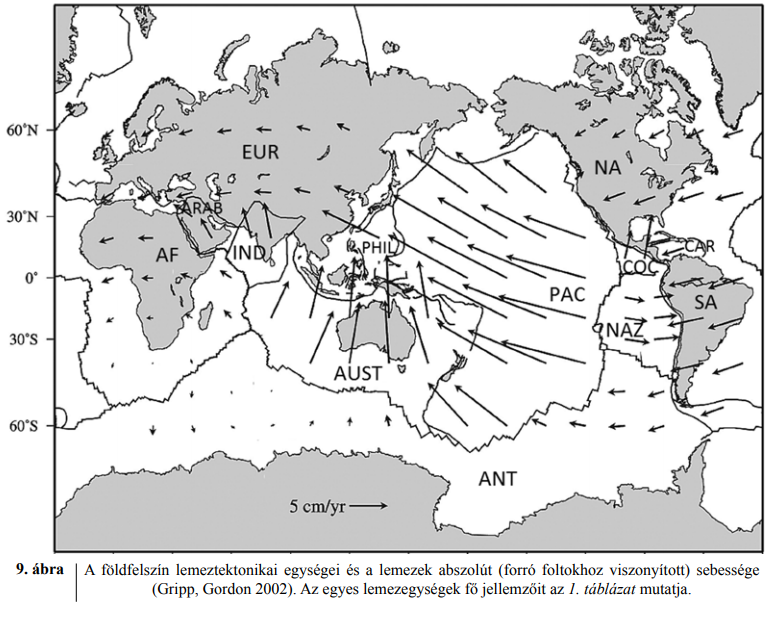
\includegraphics[width=0.75\textwidth]{wg_rel_vel_hotspot.png}
    \end{center}
\end{frame}


\begin{frame}{A lemezek mozgásának abszolút sebessége}
    \begin{center}
        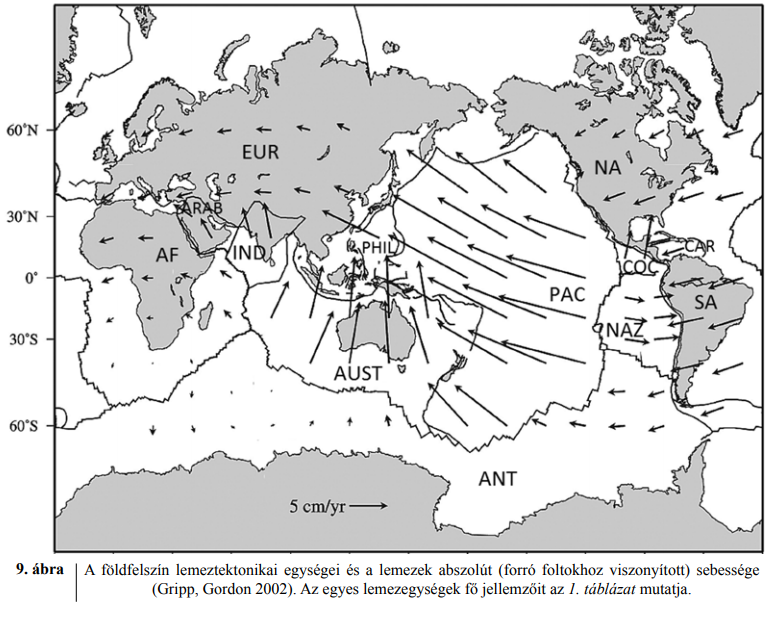
\includegraphics[width=0.675\textwidth]{wg_rel_vel_hotspot.png}
    \end{center}
    Pacifikus-lemez, teljes litoszféra rendszer mozgási energiájának 2/3-a; Pacifikus-, Indiai-Ausztrál- és Nazca-lemez a teljes energia 95\%
\end{frame}


\begin{frame}{A lemezek mozgásának abszolút sebessége}
    \begin{center}
        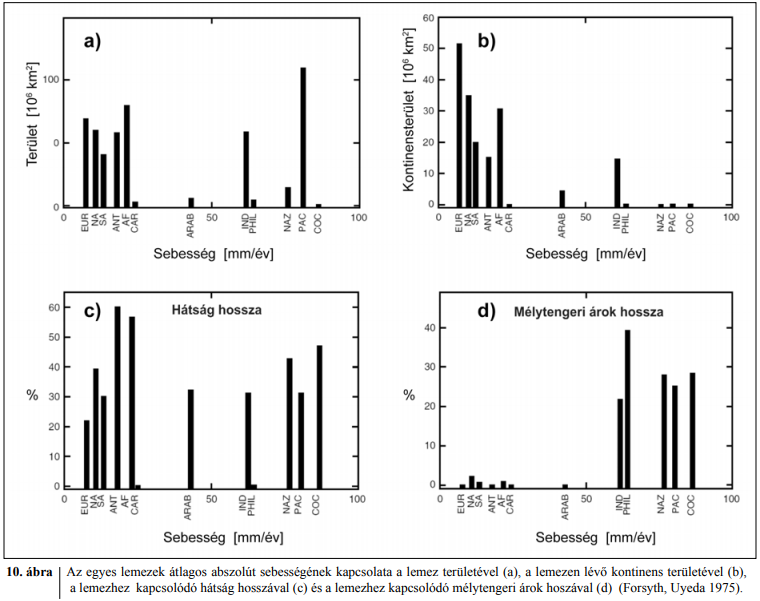
\includegraphics[width=0.7\textwidth]{wg_slab_vel_corr.png}
    \end{center}
    \begin{itemize}
        \item nincs korreláció a sebességgel: lemezméret és hátsághossz
        \item korreláció a sebességgel: kontinesterület és mélytengeri árok hossza
    \end{itemize}
\end{frame}


\begin{frame}{Új földmodell a szeizmikus tomográfia alapján}
    \begin{center}
        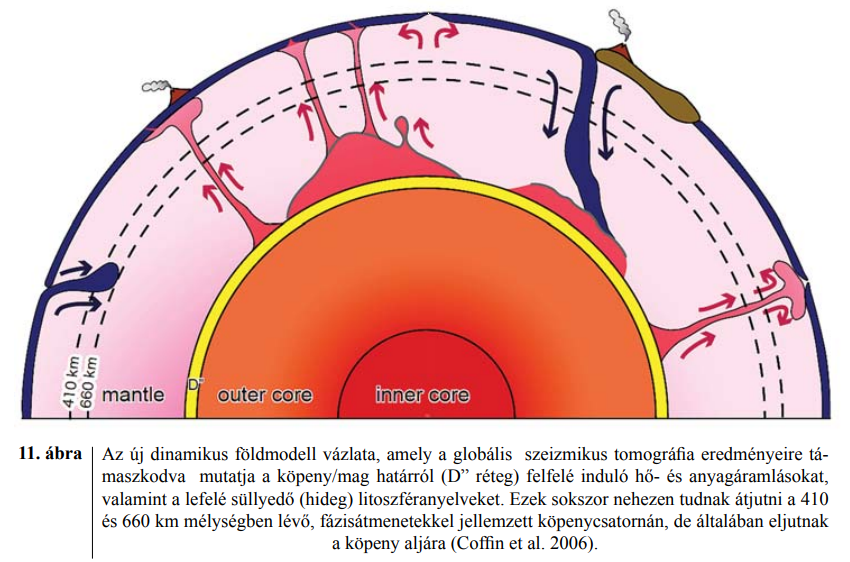
\includegraphics[width=0.7\textwidth]{wg_theory_today.png}
    \end{center}
    \begin{itemize}
        \item bazaltömlések a D'' hőáramlási oszlopokhoz kapcsolódnak
        \item leáramlások a szubdukált lemezekhez, D'' rétege érkeznek
        \item mai elképzelés szerint ez a két fő teljes köpenyre kiterjedő áramlástípus mozgatja a lemezeket
    \end{itemize}
\end{frame}

\begin{frame}{A szubdukálódó lemez és a szubdukciós zóna sematikus felépítése}
    \begin{minic}{0.825}
        \fig{bev_subd_schem.png}
    \end{minic}
\end{frame}

\begin{frame}{A szubdukció vizsgálata szeizmika segítségével}
    \begin{minipage}[c]{0.45\textwidth}
        \centering
        \inc{abers_double_seism.png}
    \end{minipage}
    \hspace{10pt}
    \begin{minipage}[c]{0.45\textwidth}
        \centering
        %\inc{SeismicTomo.jpg}
        
        Szeizmikus tomográfia szelvény a Karibi térségből.
    \end{minipage}
\end{frame}


\begin{frame}{Szeizmológiai alapok}
    \begin{minipage}[c]{0.45\textwidth}
        \begin{center}
            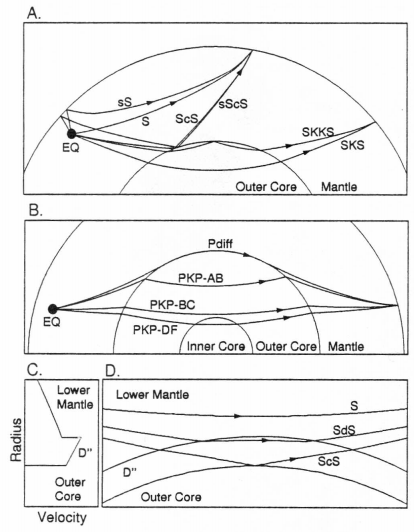
\includegraphics[width=0.85\textwidth]{wys_ray_path.png}
            
            \inc{wys_ray_path_cap.png}
        \end{center}
    \end{minipage}
    \begin{minipage}[c]{0.45\textwidth}
        \begin{itemize}
            \item P (primary, nyomás, longitudinális), S (secondary, nyírás, transzverzális) és felületi hullámok
            \item terjedési sebességük függ: közeg rugalmas tulajdonságai, sűrűség (hőméréklet)
            \item P és S hullámok egymásba alakulhatnak fázishatároknál
        \end{itemize}
        \cite{wysession}
    \end{minipage}
\end{frame}


\begin{frame}{Szeizmológiai alapok}
    \begin{figp}{\inc{helf_ray_paths.png}}{\cite{helffrich}}{0.45}{0.525}
        \begin{itemize}
            \item szeizmikus hullámok 3 módon hordoznak információt:
            \begin{itemize}
                \item hullám terjedési ideje (ismert terjedési útvonal $\rar$ átlagos útvonal menti sebesség- vagy sebesség anomália)
                \item másodlagos beérkezések $\lar$ lemez jelenléte (P $\rar$ S és S $\rar$ P diszkontinuitás a kőzet rugalmas tulajdonságaiban)
                \item frekv. függő hatások; $\lambda_i = n \cdot d_i$, $\lambda_i$-k felerősödnek/gyengülnek
            \end{itemize}
            \item szeizmológiai vizsgálatok $\rar$ sebesség (anomália) a lemez egy adott részén vagy rétegvastagság
            \item ásványtanból számított rugalmas hullám sebességek $\leftrightarrow$ szeizmikus hullám sebességek
        \end{itemize}
    \end{figp}
\end{frame}

\sepcite{Sebességkontraszt a szubdukálódó lemezben}{helffrich}

\begin{frame}{Példa - Sebességkontraszt a szubdukálódó lemezben}
    \begin{figp}{\inc{helf_japan_subd.png}}{}{0.35}{0.575}
        S $\rar$ P és P $\rar$ S fázisok; terjedési geometria és amplitúdó arányok $\rar$ konverziós réteg tulajdonságaira leírás;
        \vspace{5pt}
        
        \textbf{Pl.} alacsony sebességű réteg Észak-Honshu (Japán) alatt; 7 km vastagság, köpenyhez képest -6\%, lemezhez képest -12\%
        \vspace{20pt}
        
        ScSp fázis alapján $\rar$ helyi sebességkontraszt;
        \vspace{5pt}
        
        \textbf{Pl.} Tonga (Új-Zéland) 8-10 km vastag réteg a lemezben;
        
        \textbf{Pl.} Alaszka 2-10 km vastag réteg
        \vspace{10pt}
        
        Tonga lemez gyorsabb terjedési sebesség a köpenyhez képest, Japán és Alaszka lassabb; minden esetben a réteg $\le$ 10 km.
    \end{figp}
\end{frame}


\begin{frame}{Lemez - köpeny kontraszt}
    \textbf{alábukott lemez $\leftrightarrow$ köpeny (hőmérséklet, ásványtani összetétel):}
    \begin{itemize}
        \item hőmérsékletgradiens felszíntre merőlegesen változik leginkább, 400$^\circ$C 10 km-re a lemez felszínétől
        \item ásványtani ``kontraszt''
        \begin{itemize}
            \item lemez: olivin (ol), ortopiroxén (opx), klinopiroxén (cpx), plagioklász (pl), spinel (sp), gránát (gt)
            \item köpeny: gránát vagy spinel lherzolit
        \end{itemize}
        \item szeizmikus hullámsebességszámítások $\rar$ kízárólag a hőmérséklet- és az ásványtani kontraszt nem okozhatja az észlelt sebességkontrasztokat
    \end{itemize}
\end{frame}


\begin{frame}{Gabbró-eklogit átalakulás}
    \begin{itemize}
        \item ásványtani átalakulások $\rar$ sebességváltozás, sűrűségvaltozás a kéregben
        \item gabbró-eklogit, legsekélyebb átalakulás, +15\% sűrűségnövekedés
        \item \ce{(Mg,Fe)_2 Si O_4 (olivin) + Ca Al_2 Si_3 O_8 (anorthite) -> Ca (Mg,Fe)_2 Al_2 Si_4 O_12}
        \item felhajtőerő változás $\rar$ lefelé ``húzza'' a lemezt, földrengések a lemezben
        \item sekély átalakulás mélység (20 km)
        \item megfelelő model? ``száraz'' környezet feltételezés $\leftrightarrow$ fúrásminták hidratáltak
    \end{itemize}
\end{frame}


\begin{frame}{Szeizmikus sebesség metabazaltokban}
    \begin{minipage}[c]{0.525\textwidth}
        \centering
        \inc{helf_metabas_velo.png}
    \end{minipage}
    \hspace{10pt}
    \begin{minipage}[c]{0.4\textwidth}
        \begin{itemize}
            \item Metabazalt ásványok P sebességeinek kiszámítása $\lar$ hőmérséklet modellből
            \item kontraszt lemezfáciesekben képes sebességnövekedést előidézni a lemezrétegekben sekély alábukási szinteken
            \item észlelt sekély szeizmikus sebesség kontraszt konzisztens a számítot metabazalt sebességekkontraszttal
        \end{itemize}    
    \end{minipage}
\end{frame}

\sepcite{Kettős szeizmikus zóna}{abers}


\begin{frame}{Példa - Kettős szeizmikus zóna}
    \begin{figp}{\inc{abers_double_seism.png}}{}{0.45}{0.5}
        \begin{itemize}
            \item közepes mélységú földrengések a szubdukált kérgen kívül $\rar$ sok elméletet kizár
            \item lehetséges megoldás: második zóna $\rar$ rendellenes összetételű térrész a szubdukált köpeny litoszférán belül
            \item sok helyen észleltek kettős szeizmikus zónákat (double seismic zone - DSZ), számos szempontból hasonlóak
            \item két sáv 150-200 km-en összeér; tényleges effektus vagy artifakt? (mélységgel csökken a hipocentrum meghatározás pontossága)
        \end{itemize}
    \end{figp}
\end{frame}


\begin{frame}{Magyarázat}
    \begin{itemize}
        \item lemez görbülete $\rar$ feszültség; megfelelő megyarázat bizonyos területeken (nyugat-csendes-óceáni szubdukciós zónák)
        \item közepes mélységű földrengések fészekmechanizusai nagy ``szórás'' $\leftrightarrow$ homogén feszültségtér
        \item bazalt $\rar$ eklogit átalakulás és dehidratáció az óceáni lemezben $\leftrightarrow$ földrengések 20-40 km-el mélyebben a szubdukált köpeny litoszférában
    \end{itemize}
\end{frame}

\begin{frame}{Magyarázat}
    \begin{center}
    \begin{minipage}[c]{0.88\textwidth}
        \inc{abers_inhom_trap.png}
    \end{minipage}
    %\vspace{10pt}
    
    \begin{itemize}
        \item óceáni hátságok $\rar$ felemelkedő komplex olvadék $\rar$ litoszféra inhomogenitás; pl. mafikus magma felhalmozódása és megszilárdulása a kéreg alatt
        \item olvadék felhalmozódása nagy porozitású térrészekben
        \item földrengés? $\lar$ gázokban gazdag olvadék?
        \item nagy bizonytalanság; közvetlen mérési bizonyíték még nincs
    \end{itemize}
    \end{center}
\end{frame}

\sepcite{A szubdukciós zónák hőmérsékleti és kőzettani felépítése}{peacock}


\begin{frame}{A szubdukciós zónák hőmérsékleti és kőzettani felépítése}
    \begin{minipage}[c]{0.4\textwidth}
        \centering
        \inc{peacock_subd_schem.png}
        {\footnotesize
        \begin{itemize}
            \item $T$: hőmérséklet (K)
            \item $Q_0$: hőfluxus (W/$\text{m}^2$)
            \item $Q_{\text{sh}}$: nyírási hőtermelés (W/$\text{m}^2$)
            \item $z_f$: a vetőtől számított mélység
            \item $b$: konstans ($\approx 1$)
            \item $V$: lemezek közeledési sebessége (m/s)
            \item $\delta$: a szubdukció szöge
            \item $\kappa$: hődiffuzivitás ($\text{m}^2$/s)
        \end{itemize}
        }
    \end{minipage}
    \begin{minipage}[c]{0.5\textwidth}
        Analitikus modell ($z < $ 50 km):
        \[
            T = \frac{(Q_0 + Q_{\text{sh}}) z_f / k}{S}
        \]
        \[
            S = 1 + b \sqrt{(V z_f \sin\delta) / \kappa}
        \]
        Numerikus modell:
        \[
            \frac{\partial T}{\partial t} = \kappa \nabla^2 T - \mathbf{v} \nabla T + \frac{A}{\rho C}
        \]
        {\footnotesize
        \begin{itemize}
            \item $t$: idő (s)
            \item $\mathbf{v}$: sebességmező (m/s)
            \item $\rho$: sűrűség (kg/$\text{m}^3$)
            \item $A$: térfogati hőtermelés (W/$\text{m}^3$)
            \item $C$: hőkapacitás (J/(kg K))
        \end{itemize}
        }
    \end{minipage}
\end{frame}


\begin{frame}{Modellfuttatások eredményei}
    \begin{minipage}[c]{0.45\textwidth}
        \inc{peacock_sim_res1.png}
        
        \inc{peacock_sim_res_cap.png}
    \end{minipage}
    \begin{minipage}[c]{0.45\textwidth}
        \begin{itemize}
            \item $\delta = 26.6^\circ$
            \item $t_{\text{litoszféra}} = 50$ Ma
            \item köpenyék sebességmező $\lar$ analitikus modell
            \item stacionárius (steady-state) megoldás
            \item főbb praméterek: litoszféra hőmersékleti szerkezete (kora), közeledési sebesség, szubdukció geometriája, nyírási hőtermelés, radioaktív hőtermelés, köpenyék áramlás
            \item legfontosabb tényezők: nyírási hőtermelés, indukalt köpenyék konvekcio
        \end{itemize}
    \end{minipage}
\end{frame}


\begin{frame}{A nyírási hőtermelés szerepe}
    \begin{minipage}[c]{0.45\textwidth}
        \inc{peacock_sim_res2.png}
        
        \inc{peacock_sim_res_cap.png}
    \end{minipage}
    \begin{minipage}[c]{0.45\textwidth}
        \[
            Q_{\text{sh}} = \tau V
        \]
        \begin{itemize}
            \item $\tau$: nyírasi feszültseg (Pa)
            \item $V$: lemezek közeledési sebessége (m/s)
        \end{itemize}
        \vspace{10pt}
        
        $V$ jól ismert, $\tau$ becslés felszíni hőfluxus alapján: 0 -- néhany 10 -- $\approx$ 100 MPa
        \vspace{10pt}
        
        hőmerseklet a nyírasi zónában 100 km mélységben nyírási fűtes nélkul: 300 - 750 $^\circ$C, 100 MPa nyírási feszültség nyírasi hőtermelés: 1000 $^\circ$C
    \end{minipage}
\end{frame}



\begin{frame}{Modellek a nyírási hőtermelés kiszámitására}
    Konstans:
    \[
        \tau = \text{konstans}
    \]

    Lineáris függvénye a nyomásnak/mélységnek; töréses (súrlódásos) deformáció:
    \[
        \tau = \gamma P
    \]
    
    
    Plasztikus (creep) deformáció; jól közelíti a plasztikus anyagok reológiáját:
    \[
        \tau = \tau_{\text{BP}} \exp{[(T - T_{\text{BP}}) / L]}
    \]
    
    \begin{itemize}
        \item $\tau_{\text{BP}}$: nyírási feszültség a brittle-plastic határon
        \item $T_{\text{BP}}$: hőmérséklet a brittle-plastic határon
        \item $L$: karakterisztikus relaxációs skála
    \end{itemize}
\end{frame}


\begin{frame}{Modellfuttatások eredényei}
    \begin{minipage}[c]{0.65\textwidth}
        \centering
        \inc{peacock_mmf_facies1.png}
        \begin{itemize}
            \item ha nincs nyírási hőtermelés, gyorsabb közeledés $\rar$ kisebb szubdukciós nyírási zóna hőmérsékletek
        \end{itemize}
    \end{minipage}
    \begin{minipage}[c]{0.3\textwidth}
        \begin{itemize}
            \item nyírási hőtermelés + gyorsabb közeledés $\rar$ nagyobb hőmérsékletek
            \item fiatalabb lemez $\rar$ ``melegebb'' szubdukció
            \item indukált köpenyék könvekció $\rar$ + 200-350 $\circ$C
        \end{itemize}
    \end{minipage}
\end{frame}

\begin{frame}{Ábrafelirat}
    \begin{minic}{0.95}
        \inc{peacock_mmf_facies_cap1.png}
    \end{minic}
\end{frame}

\begin{frame}{Modellfuttatások eredényei}
    \begin{figp}{\inc{peacock_mmf_facies2.png}}{$T_{\text{BP}}$ különböző ásványokra kiszámítva: 300 $^\circ$C kvarcit, 500 $^\circ$C diabáz, márvány és kvarcit, 800 $^\circ$C olivin.}{0.65}{0.3}
        \begin{itemize}
            \item $ T > T_{\text{BP}}$ nyírási hőtermelés gyors csökkenés
            \item mérési adatok $\rar$ nyírási hőtermelés hatásának meghatározása: 10 - 30 MPa
            \item becsült hőmérséklet 100 - 125 km mélységben: 500 - 700 $\circ$C
        \end{itemize}
    \end{figp}
\end{frame}


\begin{frame}{Ábrafelirat}
    \begin{minic}{0.95}
        \inc{peacock_mmf_facies_cap2.png}
    \end{minic}
\end{frame}


\begin{frame}{Kőzettani szerkezet}
    \begin{minipage}[c]{0.45\textwidth}
        \centering
        \inc{peacock_subd_petro.png}
    \end{minipage}
    \hspace{5pt}
    \begin{minipage}[c]{0.45\textwidth}
        \begin{itemize}
            \item P-T görbék apapján $\rar$ szubdukálódó óceáni lemez nem olvad meg; szubszoliduszon keresztül kékpala $\rar$ eklogit átalakulás; ritka esetekben parciális ovladás
            \item Na-amfibol, lawsonit és klorit dehidratáviója $\rar$ nagy mennyiségű \ce{H_2 O} kibocsájtása $\rar$ parciális olvadás a köpenyékben
            \item modell bizonytalanságok $\rar$ kőzettani szerkezet bizonytalanságai
        \end{itemize}
    \end{minipage}
\end{frame}


\begin{frame}{Ábrafelirat}
    \begin{minic}{0.8}
        \inc{peacock_subd_petro_cap.png}
    \end{minic}
\end{frame}


\begin{frame}{Összefoglalás}

    {\Large
    Geofizikai megfigyelések $\rar$ modellek $\rar$ geológiai, geokémiai magyarázat
    \vspace{20pt}
    
    Modellezés $\rar$ modell pontosítása megfigyelések alapján $\rar$ geokémiai következtetések
    }
    \vspace{20pt}
    
    Megfontolások:
    \begin{itemize}
        \item Minden mérésnek, modellszámításnak (közelítések, numerikus megoldás) van hibája!
        \item Akár több modellparaméter együttes vagy modell is magyarázhatja a mérésinket.
    \end{itemize}
\end{frame}


\begin{frame}
    \begin{center}
        \Huge \color{blue!55!black}
        Köszönöm a figyelmet!
    \end{center}
\end{frame}


\begin{frame}{Irodalomjegyzék}
    {\tiny
    \bibliography{sources}
    }
\end{frame}

\end{document}
